\documentclass[12pt,a4paper]{article}
%\usepackage{fontspec, xunicode, xltxtra}  
%\setmainfont{Hiragino Sans GB}  
\usepackage{xeCJK}
%\setCJKmainfont[BoldFont=STZhongsong, ItalicFont=STKaiti]{STSong}
%\setCJKsansfont[BoldFont=STHeiti]{STXihei}
%\setCJKmonofont{STFangsong}

%使用Xelatex编译

% 设置页面
%==================================================
\linespread{2} %行距
% \usepackage[top=1in,bottom=1in,left=1.25in,right=1.25in]{geometry}
% \headsep=2cm
% \textwidth=16cm \textheight=24.2cm
%==================================================

% 其它需要使用的宏包
%==================================================
\usepackage[colorlinks,linkcolor=blue,anchorcolor=red,citecolor=green,urlcolor=blue]{hyperref} 
\usepackage{tabularx}
\usepackage{authblk}         % 作者信息
\usepackage{algorithm}     % 算法排版
\usepackage{amsmath}     % 数学符号与公式
\usepackage{amsfonts}     % 数学符号与字体
\usepackage{mathrsfs}      % 花体
\usepackage{amssymb}
\usepackage[framemethod=TikZ]{mdframed}

\usepackage{graphicx} 
\usepackage{graphics}
\usepackage{color}
\usepackage{xcolor}
\usepackage{tcolorbox}
\usepackage{lipsum}
\usepackage{empheq}

\usepackage{fancyhdr}       % 设置页眉页脚
\usepackage{fancyvrb}       % 抄录环境
\usepackage{float}              % 管理浮动体
\usepackage{geometry}     % 定制页面格式
\usepackage{hyperref}       % 为PDF文档创建超链接
\usepackage{lineno}          % 生成行号
\usepackage{listings}        % 插入程序源代码
\usepackage{multicol}       % 多栏排版
%\usepackage{natbib}         % 管理文献引用
\usepackage{rotating}       % 旋转文字,图形,表格
\usepackage{subfigure}    % 排版子图形
\usepackage{titlesec}       % 改变章节标题格式
\usepackage{moresize}   % 更多字体大小
\usepackage{anysize}
\usepackage{indentfirst}  % 首段缩进
\usepackage{booktabs}   % 使用\multicolumn
\usepackage{multirow}    % 使用\multirow

\usepackage{wrapfig}
\usepackage{titlesec}     % 改变标题样式
\usepackage{enumitem}
\usepackage{aas_macros}

\newcommand{\myvec}[1]%
   {\stackrel{\raisebox{-2pt}[0pt][0pt]{\small$\rightharpoonup$}}{#1}}  %矢量符号
\renewcommand{\vec}[1]{\boldsymbol{#1}}
\newcommand{\me}{\mathrm{e}}
\newcommand{\mi}{\mathrm{i}}
\newcommand{\dif}{\mathrm{d}}
\newcommand{\tabincell}[2]{\begin{tabular}{@{}#1@{}}#2\end{tabular}}

\def\kpc{{\rm kpc}}
\def\km{{\rm km}}
\def\cm{{\rm cm}}
\def\TeV{{\rm TeV}}
\def\GeV{{\rm GeV}}
\def\MeV{{\rm MeV}}
\def\GV{{\rm GV}}
\def\MV{{\rm MV}}
\def\yr{{\rm yr}}
\def\s{{\rm s}}
\def\ns{{\rm ns}}
\def\GHz{{\rm GHz}}
\def\muGs{{\rm \mu Gs}}
\def\arcsec{{\rm arcsec}}
\def\K{{\rm K}}
\def\microK{\mu{\rm K}}
\def\sr{{\rm sr}}
\newcolumntype{p}{D{,}{\pm}{-1}}

\renewcommand{\figurename}{Fig.}
\renewcommand{\tablename}{Tab.}

\renewcommand{\arraystretch}{1.5}

\setlength{\parindent}{0pt}  %取消每段开头的空格

\newcounter{theo}[section]\setcounter{theo}{0}
\renewcommand{\thetheo}{\arabic{section}.\arabic{theo}}
\newenvironment{theo}[2][]{%
\refstepcounter{theo}%
\ifstrempty{#1}%
{\mdfsetup{%
frametitle={%
\tikz[baseline=(current bounding box.east),outer sep=0pt]
\node[anchor=east,rectangle,fill=blue!20]
{\strut Theorem~\thetheo};}}
}%
{\mdfsetup{%
frametitle={%
\tikz[baseline=(current bounding box.east),outer sep=0pt]
\node[anchor=east,rectangle,fill=blue!20]
{\strut Theorem~\thetheo:~#1};}}%
}%
\mdfsetup{innertopmargin=10pt,linecolor=blue!20,%
linewidth=2pt,topline=true,%
frametitleaboveskip=\dimexpr-\ht\strutbox\relax
}
\begin{mdframed}[]\relax%
\label{#2}}{\end{mdframed}}

\newcommand*\widefbox[1]{\fbox{\hspace{2em}#1\hspace{2em}}}


\title{宇宙学模型2}
\author{}
\date{\today}
\begin{document}

\maketitle


\section{宇宙学红移和视界}
\cite{cheng2005relativity} The scale factor $a(t)$ is the key quantity in our description of the time evolution of the universe. In fact, because a(t) is generally a monotonic function, it can serve as a kind of cosmic clock. How can the scale factor be measured? The observable quantity that has the simplest relation to $a(t)$ is the wavelength shift of a light signal. The spectral shift is
\begin{equation}
z = \dfrac{\Delta \lambda}{\lambda} = \dfrac{\lambda_{\rm rec}}{\lambda_{\rm em}} - 1~.
\end{equation}
The wavelength (in fact any length) scales as $a(t)$, 
\begin{equation}
 \dfrac{\lambda_{\rm rec}}{\lambda_{\rm em}} =  \dfrac{ a(t_{\rm rec}) }{ a(t_{\rm em})} ~.
\end{equation}
Since the ``received time" is at $t_0$ with $a(t_0) = 1$, 
\begin{equation}
1+z = \dfrac{1}{a(t_{\rm em})} ~.
\end{equation}
At the redshift of $z = 1$, the universe had a linear size half as large as at the present one. In fact a common practice in cosmology is to refer to ``the redshift of an era" instead of its cosmic time. The ``photon decoupling time," when the universe became transparent to light is said to occur at $z = 1100$.






\cite{2010宇宙大尺度结构的形成, 2012宇宙大尺度结构的形成} 在膨胀的Friedmann宇宙中,光的传播满足
\begin{equation}
\dif \tau^2 = -g_{\mu\nu} \dif x^{\mu} \dif x^{\nu} = 0
\end{equation}
$g_{\mu\nu}$:时空度规;设光子仅沿径向(共动坐标$r$的方向)传播,即$\dif r \neq 0$,$\theta$、$\varphi$保持不变,上式化为
\begin{equation}
\dif \tau^2 = \dif t^2 -a^2(t) \frac{\dif r^2}{1-kr^2} = 0
\end{equation}
膨胀宇宙中光子传播所遵从的基本微分方程;

设某个星系位于共动坐标$r_e$处,并在时刻$t_e$发射一个光子,该光子于时刻$t_0$(现在)被位于原点处的观测者接收到,光子的波长如何变化?

设发射与接收持续的时间(周期)分别$\Delta t_e$和$\Delta  t_0$,波的开始满足
\begin{equation}
\int_{t_{e}}^{t_0} \frac{\dif t}{a(t)} = \int_0^{r_e} \frac{\dif r}{\sqrt{1-kr^2}}
\end{equation}
波的结束满足
\begin{equation}
\int\limits_{t_{e}+\Delta t_e}^{t_0 +\Delta t_0} \frac{\dif t}{a(t)} = \int_0^{r_e} \frac{\dif r}{\sqrt{1-kr^2}}
\end{equation}
因此
\begin{equation}
\int\limits_{t_{e}+\Delta t_e}^{t_0 +\Delta t_0} \frac{\dif t}{a(t)} = \int\limits_{t_{e}}^{t_0} \frac{\dif t}{a(t)} ~~\Rightarrow ~~\int\limits_{t_{e}}^{t_e+\Delta t_e} \frac{\dif t}{a(t)} = \int\limits_{t_0}^{t_0+\Delta t_0} \frac{\dif t}{a(t)} 
\end{equation}
当$\Delta t_e$和$\Delta  t_0$远小于使$a(t)$发生明显变化的时间尺度时,
\begin{equation}
\frac{\Delta t_e}{a(t_e)} = \frac{\Delta t_0}{a(t_0)} ~~\Rightarrow ~~ \frac{\Delta t_0}{\Delta t_e} = \frac{a(t_0)}{a(t_e)} 
\end{equation}
发射和接收光子的波长分别为$\lambda_e = c\Delta t_e$和$\lambda_0 = c\Delta t_0$,于是
\begin{equation}
\frac{\lambda_0}{\lambda_e} = \frac{a(t_0)}{a(t_e)}
\end{equation}
\textcolor{red}{宇宙学红移}定义为
\begin{equation}
\color{red} z \equiv \frac{\lambda_0 -\lambda_e}{\lambda_e} = \frac{a(t_0)}{a(t_e)} -1 
\end{equation}

\cite{2008cosm.book.....W} Adopt a Robertson-Walker coordinate system in which we are at the center of coordinates, and consider a light ray coming to us along the radial direction. A ray of light obeys the equation $\dif \tau^2 = 0$, for such a light ray 
\begin{equation}
\dif t = \pm a(t) \dfrac{\dif r}{\sqrt{1-kr^2}} ~.
\end{equation}
For a light ray coming toward the origin from a distant source, $r$ decreases as $t$ increases, choose the \textcolor{yellow}{minus sign}. If light leaves a source at co-moving coordinate $r_1$ at time $t_1$, it arrives at the origin $r = 0$ at a later time $t_0$, given by
\begin{equation}
\int_{t_1}^{t_0} \dfrac{\dif t}{a(t) } = \int_0^{r_1} \dfrac{\dif r}{\sqrt{1-kr^2}} ~.
\end{equation}
Taking the differential of this relation, and recalling that the radial coordinate $r_1$ of co-moving sources is time-independent, the interval $\delta {t_1}$ between departure of subsequent light signals is related to the interval $\delta {t_0}$ between arrivals of these light signals by
\begin{equation}
\dfrac{\delta t_1}{a(t_1)} = \dfrac{\delta t_0}{a(t_0)} ~.
\end{equation}
If the ``signals" are subsequent wave crests, the emitted frequency is $\nu_1 = 1/\delta t_1$, and the observed frequency is $\nu_0 = 1/\delta t_0$, 
\begin{equation}
\dfrac{\nu_0}{\nu_1} = \dfrac{a(t_1)}{a(t_0)} ~.
\end{equation}
If $a(t)$ is increasing, then this is a redshift, a decrease in frequency by $a(t_1)/a(t_0)$, equivalent to an increase in wavelength by a factor called \textcolor{red}{$1 + z$}
\begin{equation}
\color{red} 1+z = \dfrac{a(t_0)}{a(t_1)} ~.
\label{eq:1+z}
\end{equation}
If $a(t)$ is decreasing then we have a blueshift, a decrease in wavelength given by the factor Eq. (\ref{eq:1+z}) with $z$ negative. These results are frequently interpreted in terms of the familiar Doppler effect. For an increasing or decreasing $a(t)$, the \textcolor{blue}{proper distance to any comoving source of light} like a typical galaxy increases or decreases with time, so that such sources are receding from us or approaching us, which naturally produces a redshift or blueshift. Galaxies with redshift (or blueshift) $z$ are often said to have a \textcolor{yellow}{cosmological radial velocity $cz$}. (The meaning of relative velocity is clear only for $z \ll 1$, so the existence of \textcolor{yellow}{distant sources with $z > 1$ does not imply any violation of special relativity}.) However, the interpretation of the cosmological redshift as a Doppler shift  can only take us so far. The \textcolor{orange}{increase of wavelength from emission to absorption of light does not depend on the rate of change of $a(t)$ at the times of emission or absorption, but on the increase of $a(t)$ in the whole period from emission to absorption}. 

We can also understand the frequency shift by reference to the quantum theory of light: The momentum of a photon of frequency $\nu$ is $h\nu/c$ (where $h$ is Planck's constant), and this momentum varies as $1/a(t)$. 

For nearby sources, we may expand $a(t)$ in a power series, 
\begin{equation}
a(t) \simeq a(t_0) [1+(t-t_0) H_0 + \cdots ]
\end{equation}
where \textcolor{red}{$H_0$} is known as the \textcolor{red}{Hubble constant}:
\begin{equation}
H_0 \equiv \dfrac{\dot{a}(t_0) }{a(t_0)} ~.
\end{equation}
The fractional increase in wavelength is
\begin{equation}
z = H_0 (t_0 - t_1) +\cdots
\end{equation}
For close objects, $t_0 - t_1$ is the proper distance $d$ (in units with $c = 1$). We expect a redshift (for $H_0 > 0$) or blueshift (for $H_0 < 0$) that increases linearly with the proper distance $d$ for galaxies close enough to use the approximation 
\begin{equation}
z = H_0 d + \cdots 
\end{equation}
Measure the expansion rate $H(t) \equiv \dot{a}(t)/a(t)$ at times $t$ earlier than the present by observing the change in very accurately measured redshifts of individual galaxies over times as short as
a decade. The rate of change of redshift with the time of observation is
\begin{equation}
\dfrac{\dif z}{\dif t_0} = \dfrac{\dot{a}(t_0) }{a(t_1)} - \dfrac{a(t_0) \dot{a}(t_1)}{a^2(t_1)} \dfrac{\dif t_1 }{\dif t_0} =  \left[H_0 - H(t_1) \dfrac{\dif t_1 }{\dif t_0} \right] (1+z)
\end{equation}
\begin{equation}
\dfrac{\dif t_1 }{\dif t_0} = \dfrac{1}{1+z}
\end{equation}
If we measure $\dif z/\dif t_0$, the expansion rate at the time of light emission is obtained from
\begin{equation}
H(t_1) = H_0(1+z) -\dfrac{\dif z}{\dif t_0} ~.
\end{equation}






There are two different horizons, which limit the distances at which past events can be observed or at which it will ever be possible to observe future events. These are called \textcolor{red}{particle horizons} and \textcolor{red}{event horizons}, respectively. 

If the big bang started at a time $t = 0$, the greatest value \textcolor{red}{$r_{\rm max}(t)$} of the Robertson-Walker radial coordinate from which an observer at time $t$ will be able to receive signals traveling at the speed of light is given by
\begin{equation}
\int_0^t \dfrac{\dif t^\prime}{a(t^\prime)} = \int_0^{r_{\rm max}(t)} \dfrac{\dif r}{\sqrt{1-kr^2} } ~.
\label{eq:particle_hor}
\end{equation}
There is a particle horizon unless the integral $\displaystyle \int \dfrac{\dif t}{a(t)}$ does not converge at $t = 0$. It does converge in conventional cosmological theories; whatever the contribution of matter or vacuum energy at the present, it is likely that the energy density will be dominated by radiation at early times, in which case $a(t) \propto t^{1/2}$, and the integral converges. The proper distance of the horizon is 
\begin{equation}
d_{\rm max}(t) = a(t) \int_0^{r_{\rm max}(t) } \dfrac{\dif r}{\sqrt{1-kr^2} }= a(t) \int_0^t \dfrac{\dif t^\prime}{a(t^\prime)} ~.
\end{equation}
During the radiation-dominated era $a(t) \propto t^{1/2}$, so $d_{\rm max}(t) = 2t = 1/H$. Well into the matter-dominated era most of the integral over time in Eq. (\ref{eq:particle_hor}) comes from a time when $a \propto t^{2/3}$, so that $d_{\rm max}(t) \simeq 3t = 2/H$. At present most of the integral over $t$ comes from a period when the expansion is dominated by matter and the vacuum energy, and perhaps curvature as well. The particle horizon distance at present is
\begin{equation}
d_{\rm max}(t_0) = \dfrac{1}{H_0} \int_0^1 \dfrac{\dif x}{x^2 \sqrt{\Omega_\Lambda +\Omega_k x^{-2} +\Omega_Mx^{-3}} } ~.
\label{eq:proper_dis_max}
\end{equation}
There may have been a time before the radiation dominated era in which there was nothing in the universe but vacuum energy,
in which case the particle horizon distance would actually be infinite. As far as telescopic observations are concerned, Eq. (\ref{eq:proper_dis_max}) gives the \textcolor{orange}{proper distance beyond which we cannot now see}.





























\section{宇宙年龄}
\cite{perkins2008particle} The Hubble parameter at time $t$ is
\begin{align}
\nonumber H(t)^2 &= \dfrac{8\pi G}{3} \left[\rho_m(t) +\rho_r(t) +\rho_\Lambda(t) +\rho_k(t) \right] \\
\nonumber &= H_0^2 [\Omega_m(t) +\Omega_r(t) +\Omega_\Lambda(t)+\Omega_k(t)] \\
&= H_0^2[\Omega_m(0)(1+z)^3 +\Omega_r(0)(1+z)^4 +\Omega_\Lambda(0)+\Omega_k(0)(1+z)^2] 
\end{align}
where $R(0)/R(t) = (1 + z)$. Matter, radiation, and curvature terms vary as $1/R^3$, $1/R^4$, and $1/R^2$ respectively. The vacuum energy, by definition, is independent of $z$, while $\Omega_k(0) = -kc^2/(R_0H_0)^2$. 
\begin{align}
& H = \dfrac{1}{R} \dfrac{\dif R}{\dif t} = - \dfrac{\dif z/\dif t}{(1+z)} \\
& \dif t = -\dfrac{\dif z}{(1+z) H}
\end{align}
Integrate to obtain the interval from the time $t$ when the redshift was $z$, to the present time, $t_0$, when $z = 0$:
\begin{equation}
t_0 -t = \dfrac{1}{H_0} \int \dfrac{\dif z}{(1+z) [\Omega_m(0)(1+z)^3 +\Omega_r(0)(1+z)^4 +\Omega_\Lambda(0)+\Omega_k(0)(1+z)^2]^{1/2} } ~.
\end{equation}
The age is found by setting the upper limit as $z = \infty$ at $t = 0$. In the general case this integral has to be evaluated numerically, but there are a few cases where analytical solutions are possible, for example, when the radiation term can be neglected and either $\Omega_\Lambda = 0$ or $\Omega_k = 0$, as shown in Fig. \ref{fig:age_universe}.

%===========================================================================================================================
\begin{figure}
\centering
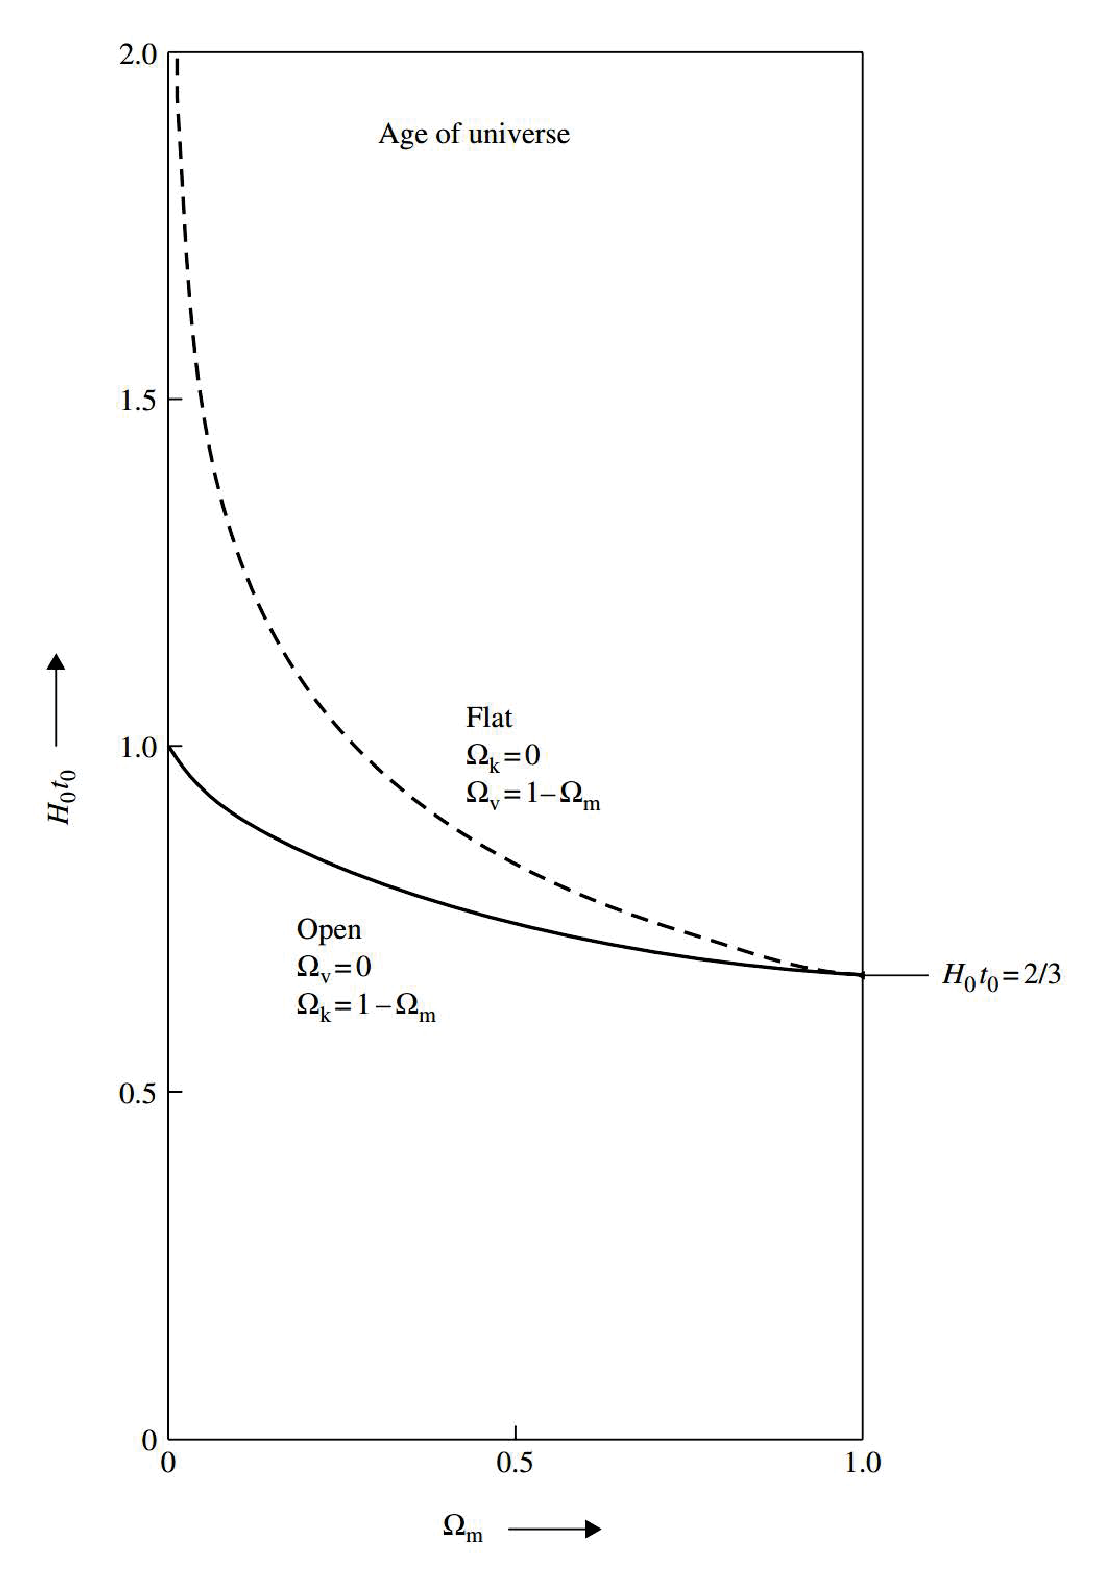
\includegraphics[height=16.cm,angle=0]{age_universe.eps}
\caption{Plot of the age of the universe versus the parameter $\Omega_m$, the ratio of the matter density to the critical density. The solid curve is for an open universe, in which the curvature term $\Omega_k = 1- \Omega_m$, and radiation and vacuum energy terms are assumed to be zero. The dashed curve is for a flat universe $(\Omega_k = 0)$, in which radiation energy is neglected and the vacuum energy $\Omega_v = 1 - \Omega_m$. The present best estimate relates to the flat universe with $\Omega_m = 0.24$.} 
\label{fig:age_universe}
\end{figure}
%===========================================================================================================================

Estimate the age of a flat universe $(k = 0)$ if radiation is neglected and it is presently made up of matter with $\Omega_m= 0.24$ and vacuum energy with $\Omega_\Lambda = 0.76$. 
\begin{align}
\nonumber H_0 t_0 &= \int_0^\infty \dfrac{\dif z}{(1+z)[\Omega (1+z)^3 +(1-\Omega)]^{1/2} } \\
&= \dfrac{1}{(1-\Omega)^{1/2}} \int_0^\infty \dfrac{\dif z}{(1+z)[\Omega (1+z)^3/(1-\Omega) +1]^{1/2} }
\end{align}
where $\Omega \equiv \Omega_m(0)$ and $\Omega_\Lambda(0) = (1-\Omega)$. 
\begin{empheq}[box=\widefbox]{align*}
\nonumber & \dfrac{\Omega(1+z)^3}{(1-\Omega)} =\tan^2 \theta \Longrightarrow \left(\dfrac{\Omega(1+z)^3}{(1-\Omega)} \right)^{1/2} =\tan \theta \\
\nonumber & \dfrac{3 \Omega (1+z)^2 \dif z }{(1-\Omega)} = \dfrac{2 \tan \theta }{\cos^2 \theta} \dif \theta \\
\nonumber & \dfrac{\Omega (1+z)^3 }{(1-\Omega)} \dfrac{\dif z }{(1+z)} = \dfrac{2 \tan \theta }{3\cos^2 \theta} \dif \theta \\
\nonumber & \dfrac{\dif z }{(1+z)} = \dfrac{2 \tan \theta }{3\cos^2 \theta} \dfrac{1}{\tan^2 \theta} \dif \theta = \dfrac{2}{3\cos^2 \theta \tan \theta} \dif \theta 
\end{empheq}
\begin{empheq}[box=\widefbox]{align*}
H_0 t_0 &= \dfrac{1}{(1-\Omega)^{1/2}} \int_0^\infty \dfrac{\dif z}{(1+z)[\Omega (1+z)^3/(1-\Omega) +1]^{1/2} } \\
&= \dfrac{1}{(1-\Omega)^{1/2}} \int_{\theta_1}^{\pi/2} \dfrac{2}{3\cos^2 \theta \tan \theta} \cos \theta \dif \theta \\
&= \dfrac{2}{3(1-\Omega)^{1/2}} \int_{\theta_1}^{\pi/2} \dfrac{1}{\sin \theta} \dif \theta \\
&= -\dfrac{2}{3(1-\Omega)^{1/2}} \int_{\theta_1}^{\pi/2} \dfrac{1}{1- \cos^2 \theta} \dif \cos \theta \\
&= -\dfrac{1}{3(1-\Omega)^{1/2}} \int_{\theta_1}^{\pi/2} \left[\dfrac{1}{1-\cos \theta} +\dfrac{1}{1+\cos \theta} \right] \dif \cos \theta \\
&= -\dfrac{1}{3(1-\Omega)^{1/2}} \left[\ln(1+\cos\theta) \Big|_{\theta_1}^{\pi/2} -\ln(1-\cos \theta) \Big|_{\theta_1}^{\pi/2} \right] \\
&= \dfrac{1}{3(1-\Omega)^{1/2}} \ln \left[\dfrac{1+\cos \theta_1}{1-\cos \theta_1} \right] = \dfrac{1}{3(1-\Omega)^{1/2}} \ln \left[\dfrac{1+(1-\Omega)^{1/2}}{1-(1-\Omega)^{1/2}} \right]
\end{empheq}
For $\Omega = 0.24$, and $1-\Omega = 0.76$, $H_0 t_0 = 1.026$, so that $t_0 = 1.026/H_0 = 13.95 \pm 0.4$ Gyr. The vacuum term has thus increased the age. 






\section{宇宙学距离}
\subsection{The proper distance}
若一个星系位于共动坐标$(r = 0, \theta, \phi)$处,另一个位于共动坐标$(r, \theta, \phi)$处,两者之间的\textcolor{red}{固有(物理)距离}:

\textcolor{red}{proper distance} $l$: for any two fundamental observers at any give cosmic time $t$,
\begin{equation}
l = a(t) \int_0^{r_1} \frac{\dif r}{\sqrt{1- kr^2}} = a(t)\chi(r_1)
\end{equation}
where
\begin{equation}
\chi(r) = \left\{
\begin{aligned}
& \sin^{-1} r,   && k = 1 \\
& r,                 && k = 0 \\
& \sinh^{-1} r, && k = -1
\end{aligned}
\right.
\end{equation}

两星系之间的相对\textcolor{red}{固有速度}:
\begin{equation}
v = \frac{\dif l}{\dif t} = \dot{a}(t) \int_0^{r} \frac{\dif r}{\sqrt{1-kr^2}} = \frac{\dot{a}}{a} \cdot l
\end{equation}

定义\textcolor{red}{哈勃常数}:
\begin{equation}
H \equiv \frac{\dot{a}}{a}
\end{equation}
\begin{equation}
v = H\cdot l
\end{equation}

$\chi(r)$: comoving distance between the two fundamental observers, the proper distance $l$ measured in units of the scale factor.

\textcolor{red}{conformal time}
\begin{equation}
\tau = \int_0^{t}  \frac{c~ \dif t'}{a(t')}
\end{equation}


\cite{cheng2005relativity} The proper distance $d_{\rm p}(\xi, t)$ to a point at the comoving radial distance $\xi$ and cosmic time $t$ can be calculated from the RW metric with $\dif \Omega = 0$ and $\dif t = 0$
\begin{equation}
d_{\rm p} (\xi ,t) = a(t) R_0 \int_0^\xi \dfrac{\dif \xi^\prime}{(1-k\xi^{\prime 2})^{1/2} } = a(t) d_{\rm p}(\xi ,t_0)~,
\end{equation}
The time dependence (due to expansion of the universe) on the RHS is entirely contained in the scale factor $a(t)$. The fixed (comoving) distance at the present epoch is
\begin{equation}
d_{\rm p} (\xi ,t_0) = R_0 \int_0^\xi \dfrac{\dif \xi^\prime}{(1-k\xi^{\prime 2})^{1/2} } = \left(\dfrac{R_0}{\sqrt{k}} \right) \sin^{-1} (\sqrt{k} \xi) ~.
\end{equation}
For a space with positive curvature $k = +1$, $d_{\rm p}(\xi, t_0) = R_0 \sin^{-1} \xi$; negative curvature, $R_0 \sinh^{-1} \xi$, and a flat space $R_0 \xi = \rho$.

To relate distance to the redshift of a light source located at the comoving distance $\xi_{\rm em}$, we use the fact that the observer and emitter are connected by a light ray along a radial path $(d\Omega = 0)$
\begin{equation}
\dif s^2 = -c^2 \dif t^2 +R_0^2 a^2(t) \dfrac{\dif \xi^2}{1-k \xi^2} = 0 ~.
\end{equation}
Moving $c^2\dif t^2$ to one side and taking the minus sign for the square-root for incoming light, 
\begin{equation}
-\int_{t_0}^{t_{\rm em}} \dfrac{c\dif t}{a(t) } = R_0 \int_0^{\xi_{\rm em}} \dfrac{\dif \xi}{\sqrt{1-k \xi^2} } = d_{\rm p}(\xi_{\rm em}, t_0)
\end{equation}
\begin{equation}
-\int_{t_0}^{t_{\rm em}} \dfrac{c\dif t}{a(t) } = -\int_1^{a_{\rm em}}  \dfrac{c\dif a}{a(t) \dot{a}(t) } = -\int_1^{a_{\rm em}} \dfrac{c~ \dif a}{a^2(t) H(t) } ~,
\end{equation}
Thus the relation between the proper distance and scale factor at the emission time is
\begin{equation}
d_{\rm p}(\xi_{\rm em}, t_0) = -\int_1^{a_{\rm em}} \dfrac{c~ \dif a}{a^2(t) H(t) } ~.
\end{equation}

The relation between proper distance and redshift in the Robertson-Walker spacetime is
\begin{equation}
d_{\rm p}(z) = -\int_1^{a_{\rm em}} \dfrac{c~ \dif a}{a^2(t) H(t) } = \int_0^z \dfrac{c ~\dif z^\prime}{H(z^\prime)} ~.
\end{equation}
where
\begin{equation}
1+z  = \dfrac{1}{a(t)} ~.
\end{equation}





\cite{perkins2008particle} The \textcolor{red}{radius of the observable universe} is determined by the \textcolor{blue}{distance to the optical horizon}, \textcolor{blue}{beyond which no light signals could reach the Earth at the present time}. As time evolves, this distance increases as more parts come inside the horizon. In a static, flat universe, the horizon distance would simply be the product
\begin{equation}
D_{\rm H} = ct_0 = 4.2 ~{\rm Gpc} ~,
\end{equation}
where $t_0$ is the age described above. A somewhat larger value would be obtained in an expanding universe. In the FLRW model of an isotropic and expanding universe with uniform curvature, the true coordinate distance to any point at time $t$ is given by $D(t) = rR(t)$, where $r$ is the co-moving coordinate distance (i.e. the distance measured on a scale expanding with the Hubble expansion) and $R(t)$ is the universal scale factor. Neither of these quantities can be measured directly. We need to express them in terms of measurable quantities, namely the Hubble parameter and the redshift $z$.

The line element in the FLRW model is
\begin{equation}
\dif s^2 = c^2 \dif t^2 -R(t)^2 \left[\dfrac{\dif r^2}{(1-kr^2)} +r^2 \dif \theta^2 +r^2 \sin^2 \theta \dif \varphi^2 \right]
\end{equation}
Consider the path of a photon to or from some distant object at fixed $(\theta, \varphi)$, for which $\dif s^2 = 0$. With $R(t) = R(0)/(1 + z)$, 
\begin{equation*}
c(1+z) \dif t = \dfrac{R(0) \dif r}{\sqrt{1-kr^2} } ~,
\end{equation*}
\begin{empheq}[box=\widefbox]{align*}
& H = \dfrac{\dot{R}}{R} = \dfrac{\dot{R}/R(0)}{R/R(0)} = -\dfrac{1}{(1+z)} \dfrac{\dif z}{\dif t} \\
& c(1+z) \dif t = -\dfrac{c \dif z}{H}
\end{empheq}
\begin{align}
& R(0) \int_0^r \dfrac{\dif r}{\sqrt{1-kr^2}} = -\int \dfrac{c \dif z}{H} = \dfrac{c I(z)}{H_0} \\
& I(z) = \int_0^z \dfrac{\dif z}{[\Omega_m(0)(1+z)^3 +\Omega_r(0)(1+z)^4 +\Omega_\Lambda(0)+\Omega_k(0)(1+z)^2]^{1/2}}
\end{align}
\begin{align}
\nonumber cI(z) /H_0 &= R(0) \sin^{-1} r  ~~~ k = +1  ~~{\rm closed} \\
\nonumber &= R(0) \sinh^{-1} r  ~~~ k = -1  ~~{\rm open} \\
&= R(0) r ~~~ k = 0 ~~{\rm flat}
\end{align}
\begin{empheq}[box=\widefbox]{align*}
\int_0^r \dfrac{\dif r}{\sqrt{1-r^2}} &= \int_0^{\theta_1} \dfrac{\dif \sin \theta}{\cos \theta} \\
&= \int_0^{\sin^{-1} r} \dif \theta \\
& = \sin^{-1} r
\end{empheq}
\begin{empheq}[box=\widefbox]{align*}
\int_0^r \dfrac{\dif r}{\sqrt{1+r^2}} &= \int_0^{\tan^{-1} r}\cos \theta \dif \tan \theta \\
&= \int_0^{\tan^{-1} r} \dfrac{1}{\cos \theta} \dif  \theta \\
& = \dfrac{1}{2} \ln \left(\dfrac{1+\sin \theta}{1-\sin \theta} \right) \\
&= \dfrac{1}{2} \ln \left(\dfrac{1+r/\sqrt{1+r^2} }{1- r/\sqrt{1+r^2} } \right) \\
x & = \ln \left(r +\sqrt{1+r^2} \right) \\
r &= \dfrac{e^x -e^{-x}}{2} = \sinh x \\
x &= \int_0^r \dfrac{\dif r}{\sqrt{1+r^2}} = \sinh^{-1} r 
\end{empheq}
The present true coordinate distance of our object at redshift $z$ is
\begin{align}
\nonumber D(z) = rR(0) &= \left[\dfrac{c}{H_0 Q} \right] \sin [I(z) Q]  ~~~ k = +1  ~~{\rm closed} \\
\nonumber &= \left[\dfrac{c}{H_0 Q} \right] \sinh [I(z) Q]  ~~~ k = -1  ~~{\rm open} \\
&= \left[\dfrac{c I(z)}{H_0 Q} \right] ~~~ k = 0 ~~{\rm flat}
\end{align}
\begin{empheq}[box=\widefbox]{align*}
\Omega_k &= -\dfrac{kc^2}{[H_0 R(0)]^2} \\
|\Omega_k(0)|^{1/2} &= \dfrac{c}{H_0 R(0)} = Q
\end{empheq}
where $Q = |\Omega_k(0)|^{1/2}$. The \textcolor{red}{horizon distance $D_{\rm H}$} is then obtained by setting the upper limit of integration as \textcolor{blue}{$z = \infty$}. For a flat, matter-dominated universe, that is, $\Omega_m(0) = 1$ and all other contributions set to zero, one obtains $D_{\rm H} = 2c/H_0$, while for a flat radiation-dominated universe with $\Omega_r(0) = 1$, $D_{\rm H} = c/H_0$.
\begin{empheq}[box=\widefbox]{align*}
I(z) &= \int_0^z \dfrac{\dif z}{[\Omega_m(0)(1+z)^3]^{1/2}} = \int_0^z \dfrac{\dif z}{(1+z)^{3/2}} \\
&= (-2) \int_0^z \dif (1+z)^{-1/2} \\
&= 2 ~~~(z \rightarrow \infty)
\end{empheq}
\begin{empheq}[box=\widefbox]{align*}
I(z) &= \int_0^z \dfrac{\dif z}{[\Omega_r(0)(1+z)^4]^{1/2}} = \int_0^z \dfrac{\dif z}{(1+z)^{2}} \\
&= (-1) \int_0^z \dif (1+z)^{-1} \\
&= 1 ~~~(z \rightarrow \infty)
\end{empheq}
For the values of the contributions to the closure parameter $\Omega_{\rm tot} = 1$, that is, $\Omega_m(0) = 0.24, \Omega_\Lambda(0) = 0.76, \Omega_r(0) = \Omega_k(0) = 0$, the integral has to be evaluated numerically. The horizon distance or visible radius of the universe is
\begin{equation}
D_{\rm H} \sim 3.3 \dfrac{c}{H_0} \sim 14 ~~{\rm Gpc} 
\end{equation}
If the dark energy term, here identified with vacuum energy, is $z$-dependent, this result would change.


\subsection{光度距离}
\cite{2010宇宙大尺度结构的形成, 2012宇宙大尺度结构的形成} 对于宇宙学距离上的遥远星系,其距离的测量目前只有两种,即光度距离和角直径距离。前者利用的是星系的绝对光度与其视光度的比较,后者利用的是星系的真直径与其观测到的角直径的比较。

在静态的欧几里德空间,如果一个星系的真实光度是$L$ , 观测到的辐射流量(照度)是$f$,则
\begin{equation}
f =\dfrac{L}{4\pi D^2} ~,
\end{equation}
$D$是欧氏空间中的星系距离。当空间不是静态的欧氏空间时,光度距离$D_L$为
\begin{equation*}
f =\dfrac{L}{4\pi D_L^2} \rightarrow D_L = \left(\dfrac{L}{4\pi f} \right)^{1/2}
\end{equation*}
设观测者位于共动坐标系的原点即$r=0$处,星系的共动坐标是$r_e$,光子发射的时刻是$t_e$,接收到的时刻是$t_0$。此时,波前的面积是
\begin{equation}
A = 4\pi r_e^2 a^2(t_0) ~.
\end{equation}
有两个因素使得穿过波前的辐射能流减小:1. 光子的红移,使得每个光子的能量变为$h \nu_0 = h \nu_e/(1+z)$; 2. 时间膨胀,使得单位时间内到达观测者的光子数减小一个因子$1/(1+z)$。总的效果是使到达观测者的辐射能流减小一个因子$1/(1+z)^2$。故观测者接收到的辐射流量就是
\begin{equation}
f = \dfrac{L}{4\pi r_e^2 a^2(t_0) (1+z)^2} = \dfrac{L a^2(t_e)}{4\pi r_e^2 a^4(t_0)} ~,
\end{equation}
光度距离为
\begin{equation}
D_L = \dfrac{r_e a^2(t_0)}{a(t_e)} = r_e a(t_0) (1+z) ~.
\end{equation}
这一距离并不等于固有(物理)距离。只有在$r_e$很小($z$很小)的情况下,这两者才趋于一致。光度距离测量的关键是如何确定 $r_e a(t_0)$。
\begin{equation}
r(z) = S\left[\int\limits_{t(z)}^{t_0} \dfrac{\dif t}{a(t)} \right] = S\left[\dfrac{1}{a(t_0) H_0} \int\limits_{1/(1+z)}^{1} \dfrac{\dif a}{a^2 \sqrt{\Omega_\Lambda +\Lambda_k a^{-2} +\Omega_m a^{-3} +\Omega_r a^{-4} } } \right]
\end{equation}
$S$的定义
\begin{equation}
S(y) \equiv \left\{
\begin{aligned}
& \sin y ~~~ (k = +1) \\
& y ~~~ (k = 0) \\
& \sinh y ~~~ (k = -1)
\end{aligned}
\right.
\end{equation}
当$k=0$,再利用变换$a(t) =1/(1+z)$井忽略$\Omega_{r}$项,
\begin{equation}
r(z) = \dfrac{1}{a(t_0) H_0} \int_0^z  \dfrac{\dif z}{\sqrt{\Omega_\Lambda  +\Omega_m (1+z)^{3} } } ~,
\end{equation}

\begin{equation}
D_L = r_e a(t_0) (1+z) = \dfrac{c(1+z)}{H_0} \int_0^z \dfrac{\dif z}{\sqrt{\Omega_\Lambda  +\Omega_m (1+z)^{3} } } ~.
\end{equation}

\cite{2008cosm.book.....W} At the time $t_0$ that the light reaches earth, the proper area of a sphere drawn around the luminous object and passing through the earth is given by the metric
\begin{align}
\nonumber & \dif \tau^2 \equiv -g_{\mu \nu}(x) \dif x^\mu \dif x^\nu = \dif t^2 -a^2(t) \left[\dif \vec{x}^2 +K \dfrac{(\vec{x} \cdot \dif \vec{x})^2}{1-k \vec{x}^2 }  \right] ~, \\
\nonumber & g_{ij} = a^2(t) \left(\delta_{ij} +k \dfrac{x^i x^j}{1-k \vec{x}^2} \right) ~, ~~~~ g_{i0} = 0 ~, ~~~ g_{00} = -1 ~,
\end{align}
as $4 \pi r_1^2 a^2(t_0)$, where $r_1$ is the coordinate distance of the earth as seen from the luminous object, which is the same as the coordinate distance of the luminous object as seen from the earth. The fraction of the light received in a telescope of aperture $A$ on earth is $A/4\pi r_1^2 a^2(t_0)$, and so the factor $1/d^2$ in the formula for must be replaced with $1/r_1^2 a^2(t_0)$.

The rate of arrival of individual photons is lower than the rate at which they are emitted by the redshift factor $a(t_1)/a(t_0) = 1/(1+z)$.

The energy $h\nu_0$ of the individual photons received on earth is less than the energy $h \nu_1$ with which they were emitted by the same redshift factor $1/(1+z)$.

The apparent luminosity of a source at radial coordinate $r_1$ with a redshift $z$ of any size
\begin{equation}
\ell =\dfrac{L}{4\pi r_1^2 a^2(t_0) (1+z)^2 } ~.
\end{equation}

The luminosity distance $d_L$ is 
\begin{equation}
\ell = \dfrac{L}{4\pi d_L^2} ~.
\end{equation}
\begin{equation}
d_L = a(t_0) r_1 (1+z) ~.
\end{equation}
For objects with $z \ll 1$, write the relation between luminosity distance and redshift as a power series. The redshift $1+ z \equiv a(t_0)/a(t_1)$ is related to the ``look-back time" $t_0 - t_1$ by
\begin{equation}
z = H_0 (t_0 -t_1) + \dfrac{1}{2} (q_0 +2 ) H_0^2 (t_0 -t_1)^2 + \cdots 
\end{equation}
where $H_0$ is the Hubble constant and $q_0$ is the deceleration parameter
\begin{equation}
q_0 \equiv -\dfrac{1}{H_0^2 a(t_0)} \dfrac{\dif^2 a(t)}{\dif t^2} \Big|_{t=t_0} ~.
\end{equation}
This can be inverted, to give the look-back time as a power series in the redshift
\begin{equation}
H_0 (t_0 -t_1) = z - \dfrac{1}{2} (q_0 +2) z^2 +\cdots 
\end{equation}
The coordinate distance $r_1$ of the luminous object is 
\begin{equation}
\dfrac{t_0 -t_1}{a(t_0) } + \dfrac{H_0(t_0 -t_1)^2}{2a(t_0) }  + \cdots = r_1 + \cdots ~,
\end{equation}
with the dots on the right-hand side denoting terms of third and higher order in $r_1$.
\begin{equation}
r_1 a(t_0) H_0 = z - \dfrac{1}{2} (1+q_0) z^2 + \cdots ~.
\end{equation}
This gives the luminosity distance as a power series
\begin{equation}
d_L = H_0^{-1} \left[ z + \dfrac{1}{2} (1-q_0) z^2 + \cdots  \right] ~.
\label{eq:dL_power}
\end{equation}
We can measure $q_0$ as well as $H_0$ by measuring the luminosity distance as a function of redshift to terms of order $z^2$. The same reasoning has been used to extend the expression (\ref{eq:dL_power}) to fourth order in $z$
\begin{align}
\nonumber d_L(z) = & H_0^{-1} \left[z + \dfrac{1}{2} (1-q_0) z^2 - \dfrac{1}{6} \left(1-q_0 -3q_0^2 +j_0 +\dfrac{k}{H_0^2 a_0^2} \right) z^3  \right. \\
& \left.  +\dfrac{1}{24} \left(2-2q_0-15 q_0^2 -15q_0^3 +5j_0 +10 q_0 j_0 +s_0 + \dfrac{2k(1+3q_0)}{H_0^2 a_0^2} \right) z^4 +\cdots \right] ~,
\end{align}
where \textcolor{red}{$j_0$} and \textcolor{red}{$s_0$} are parameters known as the \textcolor{red}{jerk} and \textcolor{red}{snap}:
\begin{align*}
j_0 \equiv \dfrac{1}{H_0^3 a(t_0)} \dfrac{\dif^3 a(t)}{\dif t^3} \Big|_{t=t_0} ~, \\
s_0 \equiv \dfrac{1}{H_0^4 a(t_0)} \dfrac{\dif^4 a(t)}{\dif t^4} \Big|_{t=t_0} ~.
\end{align*}





































\subsection{角直径距离}
\cite{2010宇宙大尺度结构的形成, 2012宇宙大尺度结构的形成} 角直径距离是用测量到的星系角直径与星系真实(固有)大小的关系而定义的,
\begin{equation}
D_A = a(t_e) r_e = a(t_0) r_e \dfrac{a(t_e)}{a(t_0)} = a(t_0) r_e (1+z)^{-1} 
\end{equation}
它与光度距离之间满足
\begin{equation}
D_A = D_L (1+z)^{-2} = \dfrac{c}{H_0(1+z)} \int_0^z \dfrac{\dif z}{\sqrt{\Omega_\Lambda  +\Omega_m (1+z)^{3} } } ~.
\end{equation}
当红移$z \ll 1$时,我们可以把光度距离和角直径距离中的被积函数展开为$z$的级数,并只保留有限的项。例如通常把被积函数分母中的参数$\Omega_A$换成减速因子$q_0$。并在积分后保留至$z^3$的项。积分结果为
\begin{equation}
\left[ \int\limits_0^z \right] = z - \dfrac{1}{2}(1+q_0) z^2 +\dfrac{1}{6} \left(2+5q_0 +3q_0^2 -\dfrac{3}{2} \Omega_m \right) z^3 ~.
\end{equation}
$D_L$保留至$z^3$的结果为
\begin{equation}
D_L = \dfrac{c}{H_0} \left[ z +\dfrac{1}{2}(1-q_0) z^2 -\dfrac{1}{6} \left(1-2q_0 -3q_0^2 +\dfrac{3}{2} \Omega_m \right) z^3 \right] ~.
\end{equation}

\cite{2008cosm.book.....W} A source at co-moving radial coordinate $r_1$ that emits light at time $t_1$ and is observed at present to subtend a small angle $\theta$ will extend over a proper distance s (normal to the line of sight) equal to $a(t_1)r_1 \theta$. The angular diameter distance $\dif A$ is defined so that $\theta$ is given by the usual relation of Euclidean geometry
\begin{equation}
\theta = s/d_A ~,
\end{equation}
and
\begin{equation}
d_A = a(t_1) r_1 ~.
\end{equation}
The ratio of the luminosity and angular-diameter distances is a function of redshift
\begin{equation}
\dfrac{d_A}{d_L} = (1+z)^{-2} ~.
\end{equation}
If we have measured the luminosity distance at a given redshift (and if we are convinced of the correctness of the Robertson-Walker metric), then we learn nothing additional about $a(t)$ if we also measure the angular diameter distance at that redshift. Neither galaxies nor supernovas have well-defined edges, so angular diameter distances are much less useful in studying the cosmological expansion than are luminosity distances. The observation of acoustic oscillations in the matter density may allow a measurement of yet another distance, a \textcolor{red}{structure distance}, equal to \textcolor{red}{$a(t_0)r_1 = (1+z)d_A$}.



\section{Number counts}
\cite{2015eaci.book.....S} Consider now a population of sources with a luminosity function that is constant in space and time, i.e., let $n(> L)$ be the spatial number density of sources with luminosity larger than $L$. A spherical shell of radius $r$ and thickness dr around us contains $4 \pi r^2 \dif r n(> L)$ sources with luminosity larger than $L$. Because the observed flux $S$ is related to the luminosity via $L = 4 \pi r^2 S$, the number of sources with flux $> S$ in this spherical shell is given as $\dif N(> S) = 4\pi r^2 \dif r n(> 4\pi r^2 S)$, and the total number of sources with flux $> S$ results from integration over the radii of the spherical shells
\begin{equation}
N(>S) = \int_0^\infty \dif r 4\pi r^2 n (> 4\pi r^2 S) ~.
\end{equation}
Changing the integration variable to $L = 4\pi r^2 S$, or $r = \sqrt{L/(4\pi S)}$, with $\dif r = \dif L/(2\sqrt{4\pi LS})$, yields
\begin{align}
\nonumber N(> S) &= \int_0^\infty \dfrac{\dif L}{2\sqrt{4\pi LS}} \dfrac{L}{S} n(> L) \\
&\propto S^{-3/2} \int_0^\infty \dif L \sqrt{L} n(> L) ~.
\end{align}
The source counts in such a universe is $N(> S) \propto S^{-3/2}$, independent of the luminosity function. This is in contradiction to the observations. 










\cite{2008cosm.book.....W}

















































%%%%%%%%%%%%%%%%%%%%%%%%%%%%%%%%%%%%%%%%%%%%%%%%%%%%%%%%%%%%%%%%%%%%%%
\bibliographystyle{unsrt_update}
\bibliography{ref}
%%%%%%%%%%%%%%%%%%%%%%%%%%%%%%%%%%%%%%%%%%%%%%%%%%%%%%%%%%%%%%%%%%%%%%


\end{document}
